% This file was created by matlab2tikz.%
%
\definecolor{mycolor1}{rgb}{0.90196,0.62353,0.00000}%
\definecolor{mycolor2}{rgb}{0.00000,0.61961,0.45098}%
\definecolor{mycolor3}{rgb}{0.00000,0.44706,0.69804}%
\definecolor{mycolor4}{rgb}{0.19608,0.19608,0.19608}%
%
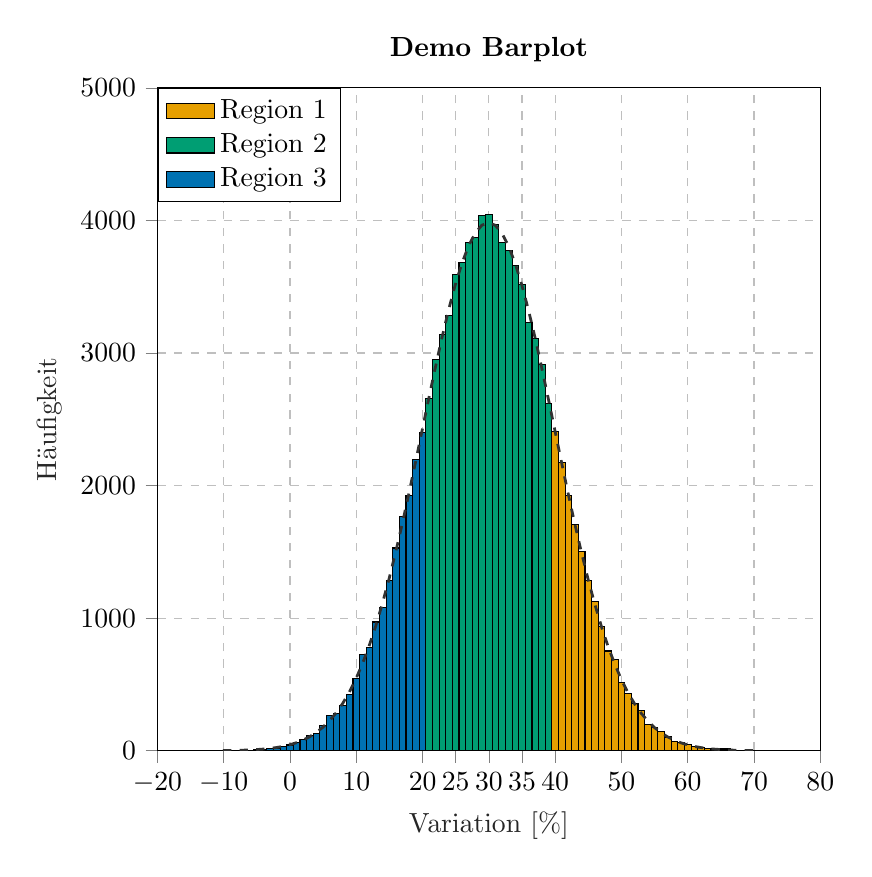
\begin{tikzpicture} 
\pgfplotsset{legend image code/.code={\draw [#1] (0cm,-0.1cm) rectangle (0.6cm,0.1cm);},}

\begin{axis}[%
%bar shift auto,
xmin=-20,
xmax=80,
xtick={-20, -10,   0,  10,  20,  25,  30,  35,  40,  50,  60,  70,  80},
tick align=outside,
xlabel style={font=\color{white!15!black}},
xlabel={Variation [\%]},
ymin=0,
ymax=5000,
ylabel style={font=\color{white!15!black}},
ylabel={Häufigkeit},
axis background/.style={fill=white},
title style={font=\bfseries},
title={Demo Barplot},
xmajorgrids,
xminorgrids,
ymajorgrids,
yminorgrids,
grid style={dashed},
x tick label style={/pgf/number format/.cd, fixed, fixed zerofill, precision=0, /tikz/.cd},
y tick label style={/pgf/number format/.cd, fixed, fixed zerofill, precision=0, /tikz/.cd},
xtick={-20,-10,0,10,20,25,30,35,40,50,60,70,80},
ytick={0,1000,2000,3000,4000,5000},
ytick pos=left,
xtick pos=bottom,
/pgf/number format/.cd, set decimal separator={.},
/pgf/number format/.cd, 1000 sep={},
legend style={at={(0,1)}, anchor=north west},
legend cell align={left},
at={(0cm,0cm)},
height=10cm,
width=10cm
]
\addplot[ybar, bar width=1, fill=mycolor1, draw=black] table[row sep=crcr] {%
40	2409\\
41	2174\\
42	1922\\
43	1704\\
44	1505\\
45	1281\\
46	1128\\
47	935\\
48	752\\
49	688\\
50	513\\
51	432\\
52	356\\
53	306\\
54	199\\
55	172\\
56	142\\
57	104\\
58	73\\
59	61\\
60	44\\
61	31\\
62	25\\
63	18\\
64	14\\
65	13\\
66	13\\
67	4\\
68	4\\
69	1\\
70	3\\
};
\addplot [color=black, forget plot]
  table[row sep=crcr]{%
-20	0\\
80	0\\
};
\addplot[ybar, bar width=1, fill=mycolor2, draw=black] table[row sep=crcr] {%
21	2658\\
22	2952\\
23	3142\\
24	3280\\
25	3589\\
26	3686\\
27	3834\\
28	3872\\
29	4040\\
30	4046\\
31	3968\\
32	3834\\
33	3774\\
34	3663\\
35	3519\\
36	3230\\
37	3110\\
38	2913\\
39	2619\\
};
\addplot [color=black, forget plot]
  table[row sep=crcr]{%
-20	0\\
80	0\\
};
\addplot[ybar, bar width=1, fill=mycolor3, draw=black] table[row sep=crcr] {%
-10	2\\
-9	1\\
-8	3\\
-7	5\\
-6	1\\
-5	12\\
-4	9\\
-3	14\\
-2	21\\
-1	29\\
0	43\\
1	64\\
2	85\\
3	112\\
4	130\\
5	189\\
6	265\\
7	283\\
8	344\\
9	424\\
10	544\\
11	727\\
12	776\\
13	971\\
14	1083\\
15	1285\\
16	1529\\
17	1769\\
18	1922\\
19	2200\\
20	2403\\
};
\addplot [color=black, forget plot]
  table[row sep=crcr]{%
-20	0\\
80	0\\
};
\addplot [color=mycolor4, dashed, line width=1.0pt, forget plot]
  table[row sep=crcr]{%
-10.1089970806553	1.33646787696355\\
-9.10762452190028	1.98383178823833\\
-8.10625196314528	2.91546760732525\\
-7.10487940439028	4.24198033825572\\
-6.10350684563528	6.11063209955091\\
-5.10213428688028	8.71486528581093\\
-4.10076172812529	12.3053019348266\\
-3.09938916937029	17.2020785270503\\
-2.09801661061529	23.8082038560051\\
-1.09664405186029	32.6234130108532\\
-0.0952714931052938	44.2577377739221\\
0.906101065649706	59.44373417998\\
1.9074736244047	79.0460205222841\\
2.9088461831597	104.066510743802\\
3.9102187419147	135.643513644645\\
4.9115913006697	175.042748478762\\
5.9129638594247	223.638346178429\\
6.91433641817969	282.882105106016\\
7.91570897693469	354.259686228439\\
8.91708153568969	439.233086585794\\
9.91845409444469	539.169623145204\\
10.9198266531997	655.258766589894\\
11.9211992119547	788.41943101629\\
12.9225717707097	939.201664301824\\
13.9239443294647	1107.68797995986\\
14.9253168882197	1293.40068822058\\
15.9266894469747	1495.22237579488\\
16.9280620057297	1711.33700988241\\
17.9294345644847	1939.19888542426\\
18.9308071232397	2175.53571972658\\
19.9321796819947	2416.39060710815\\
20.9335522407497	2657.20532855002\\
21.9349247995047	2892.94479091433\\
22.9362973582597	3118.25933951081\\
23.9376699170147	3327.67859452926\\
24.9390424757697	3515.82758770643\\
25.9404150345247	3677.65360737658\\
26.9417875932797	3808.65055793722\\
27.9431601520347	3905.06700584683\\
28.9445327107897	3964.08453583491\\
29.9459052695446	3983.95459225921\\
30.9472778282997	3964.08453583491\\
31.9486503870547	3905.06700584683\\
32.9500229458096	3808.65055793722\\
33.9513955045646	3677.65360737658\\
34.9527680633196	3515.82758770643\\
35.9541406220746	3327.67859452925\\
36.9555131808296	3118.25933951081\\
37.9568857395846	2892.94479091433\\
38.9582582983396	2657.20532855002\\
39.9596308570946	2416.39060710815\\
40.9610034158496	2175.53571972658\\
41.9623759746046	1939.19888542426\\
42.9637485333596	1711.33700988241\\
43.9651210921146	1495.22237579488\\
44.9664936508696	1293.40068822058\\
45.9678662096246	1107.68797995985\\
46.9692387683796	939.201664301822\\
47.9706113271346	788.419431016289\\
48.9719838858896	655.258766589894\\
49.9733564446446	539.169623145203\\
50.9747290033996	439.233086585793\\
51.9761015621546	354.259686228439\\
52.9774741209096	282.882105106016\\
53.9788466796646	223.638346178428\\
54.9802192384196	175.042748478762\\
55.9815917971746	135.643513644644\\
56.9829643559296	104.066510743802\\
57.9843369146846	79.0460205222838\\
58.9857094734396	59.44373417998\\
59.9870820321946	44.2577377739219\\
60.9884545909496	32.6234130108531\\
61.9898271497046	23.8082038560051\\
62.9911997084596	17.2020785270503\\
63.9925722672146	12.3053019348266\\
64.9939448259696	8.71486528581092\\
65.9953173847246	6.11063209955091\\
66.9966899434796	4.2419803382557\\
67.9980625022346	2.91546760732525\\
68.9994350609896	1.98383178823833\\
70.0008076197446	1.33646787696355\\
};
\legend{Region 1, Region 2, Region 3}% 
\end{axis}%
\end{tikzpicture}%